% !TEX root = ./informe.tex

\section{Greedy}

\subsection{Explicación}

Vimos que construir la mejor solución de forma exacta es algo que, en la práctica, es completamente inútil por su complejidad temporal. Consideremos entonces la siguiente heurística: teniendo un conjunto solución $S$ que forma una clique, en cada paso podemos golosamente agregar a $S$ el mejor nodo que haga aumentar el tamaño de la frontera. \\

Intuitivamente es un algoritmo rápido, pues en cada iteración principal tomamos un nodo que forme clique con lo que ya tenemos, y ya no quitamos ese nodo. Además, parece razonable que el algoritmo encuentre soluciones buenas: en cada iteracion estamos maximizando la frontera con el mejor nodo posible. Luego de presentar el algoritmo veremos qué tan buena era nuestra intuición. \\

Mas detalladamente, el algoritmo funciona de la siguiente manera: \\

Primero consideramos que todos los nodos son candidatos, y vamos a ejecutar el algoritmo siempre que exista algún candidato en la lista. Además mantenemos un vector $S$ que representa la solución actual, inicialmente vacío. Consideramos que nuestra frontera máxima $FM$ inicia con valor $-1$. \\

Para cada iteración del ciclo principal, queremos agregar el mejor candidato posible a la solución. Esto significa iterar por todos los candidatos y agregar a la solución aquel que maximice la frontera. \\

Recorremos la lista de candidatos y tomamos $c$ alguno. Consideramos $c$ como parte de la solución. Si la solución $S$ no forma una clique, entonces quitamos $c$ de $S$ , consideramos que ya no es más un candidato y volvemos al comienzo del algoritmo. Si $S$ forma una clique, entonces calculamos su frontera $f$. \\

Comparamos la frontera $f$ con la frontera máxima $FM$. Si $f < FM$, entonces quitamos a $c$ de $S$, pues no hace que la solución mejore. Si $f \geq FM$, entonces mantenemos a $c$, ahora $c$ es nuestro mejor candidato, pues la frontera máxima no empeoró. Actualizamos $FM$ con el valor de $f$. En ambos casos quitamos también a $c$ de la lista de candidatos, para no repetirlo dos veces. \\

Una vez encontrado el $c$ que maximice la solución, lo agregamos definitivamente y seguimos iterando hasta que ya no se pueda considerar más candidatos. \\

Finalizado el algoritmo, $S$ es una clique elegida de manera golosa, con la mayor frontera que se puedo encontrar. \\


\subsection{Pseudocódigo}

Referencias de variables globales para el pseudocódigo:
\begin{itemize}
    \item $n$: La cantidad de nodos
    \item $solucion$: Secuencia que contiene la clique solución
    \item $candidatos$: Secuencia con los nodos a considerar
    \item $fronteraMax$: El cardinal de la frontera de la clique solución
\end{itemize}

Las funciones ``EsClique()'' y ``Frontera()'' son las mismas que en el algoritmo exacto. Dado que se usan en todos los algoritmos, son omitidas. Tienen complejidad $O(n^3)$ y $O(n^2)$ respectivamente.

\begin{algorithm}[H]
\begin{algorithmic}
\Function{Resolver}{}
    \State LeerInput()                              \Comment $O(n^2)$
    \State $solucion \gets \emptyset$               \Comment $O(1)$
    \State $candidatos \gets \{1, 2, 3, .. , n\} $  \Comment $O(n)$
    \State $fronteraMax \gets -1$                   \Comment $O(1)$
    \State ObtenerSolucion()                        \Comment $O(n^5)$
\EndFunction
\end{algorithmic}
\end{algorithm}



\begin{algorithm}[H]
\begin{algorithmic}
\Function{ObtenerSolucion}{}

    \While{$candidatos \neq \emptyset$}             \Comment $O(n^5)$

        \State $mejorCandidato \gets -1$            \Comment $O(1)$

        \For{$c \in candidatos$}                    \Comment $O(n^4)$
            \State $solucion.push(c)$               \Comment $O(1)$

            \If {$\neg$EsClique($solucion$)}                        \Comment $O(n^3)$
                \State $solucion.erase(c)$                          \Comment $O(n)$
                \State $candidatos.erase(c)$                        \Comment $O(n)$
            \Else
                \State $fronteraActual \gets$ Frontera($solucion$)  \Comment $O(n^2)$
                \If{$fronteraActual \geq fronteraMax$}              \Comment $O(1)$
                    \State $fronteraMax \gets fronteraActual$       \Comment $O(1)$
                    \State $mejorCandidato \gets c$                 \Comment $O(1)$
                \Else
                    \State $candidatos.erase(c)$                    \Comment $O(n)$
                \EndIf

                \State $solucion.erase(c)$                          \Comment $O(n)$
            \EndIf
        \EndFor

        \If{$mejorCandidato \neq -1$}                               \Comment $O(1)$
            \State $solucion.push(mejorCandidato)$                  \Comment $O(1)$
            \State $candidatos.erase(mejorCandidato)$               \Comment $O(n)$

        \EndIf
    \EndWhile

    \State return $solucion$

\EndFunction

\end{algorithmic}
\end{algorithm}

\subsection{Complejidad}

La complejidad principal del algoritmo se encuentra en ``ObtenerSolucion()'', que es $O(n^5)$. Esto es fácil de ver: como nunca se agregan candidatos y siempre se quita al menos uno, el ciclo exterior se ejecuta a lo sumo $O(n)$ veces. El $For$ recorre la lista de candidatos, que son también a lo sumo $O(n)$. Dentro del $For$ encontramos solo dos funciones grandes, ``EsClique'' de $O(n^3)$ y ``Frontera'' de $O(n^2)$. El resto son comparaciones, asignaciones y borrados, de $O(n)$. \\

Más intuitivamente, EsClique ($O(n^3)$) se ejecuta $O(n)$ veces en el For, y a su vez se ejecuta $O(n)$ veces en el While. Por lo tanto, es $O(n^5)$. \\

Si bien $O(n^5)$ puede parecer un polinomio ``grande'', es exponencialmente mejor que el algoritmo exacto que tenía $O(2^{n} * n^{3})$. El trade-off es que no siempre se producen soluciones óptimas. \\

\subsection{Optimalidad}

Como podrá verse más adelante, las soluciones para grafos aleatorios son bastante buenas, pero existe al menos un tipo específico de grafos donde la diferencia entre el exacto y el greedy puede ser \textbf{arbitrariamente grande}. \\

Veamos como podemos construir este tipo de grafos. \\

{\centering
    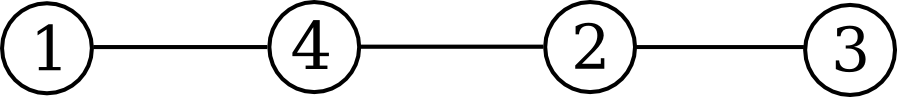
\includegraphics[width=0.57\textwidth]{informe/imgs/greedy_base.png} \\
    \captionof{figure}{Grafo inicial}
}

$ $\newline

Agreguemos 6 vecinos al nodo 1 y agreguemos 4 vecinos a los nodos 2 y 3. El algoritmo goloso toma el primer nodo como solución inicial, es el que tiene más vecinos. Luego intenta agregar nodos a la solución de forma tal que formen clique y que tengan mayor frontera. Esto no puede suceder: lo mejor que puede obtener el algoritmo goloso es una clique con frontera de tamaño 7. Sin embargo, podemos ver que la solución óptima está formada por la clique con los nodos 2 y 3, con una frontera de tamaño 9.\\

{\centering
    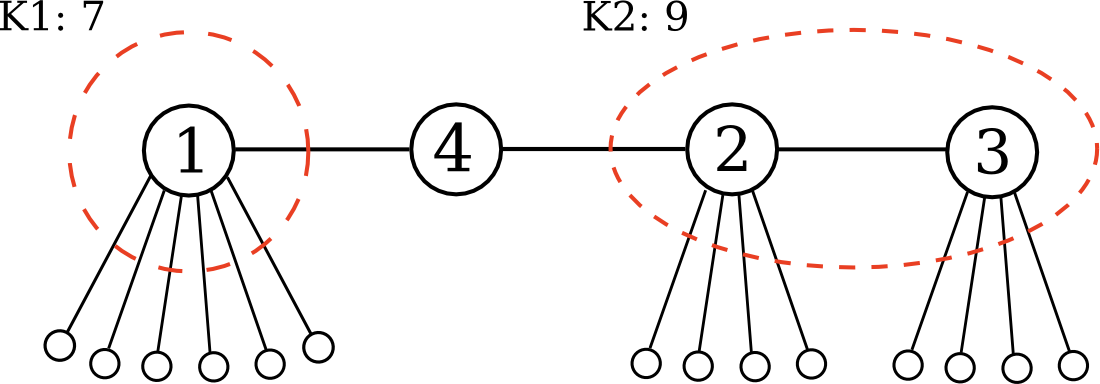
\includegraphics[width=0.57\textwidth]{informe/imgs/greedy_base_nodes_v1.png} \\
}
$ $\newline

Este es un procedimiento que podemos seguir repitiendo. Agregamos un vecino al nodo 1, y un vecino a los nodos 2 y 3. La frontera máxima golosa aumenta en 1, mientras que la frontera máxima aumenta en 2. De esta forma, podemos construir grafos donde la diferencia entre la solución óptima y la solución golosa sea arbitrariamente grande. Haremos una demostración más formal al final de la sección.\\

{\centering
    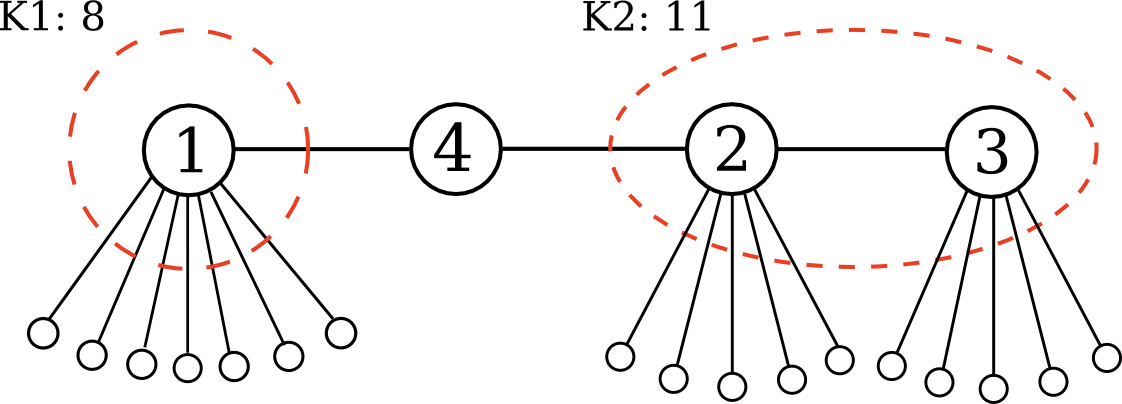
\includegraphics[width=0.57\textwidth]{informe/imgs/greedy_base_nodes_v2.png} \\
}

\subsection{Experimentación}

% Innecesarios, con uno solo de tiempo es suficiente
% {\centering
%     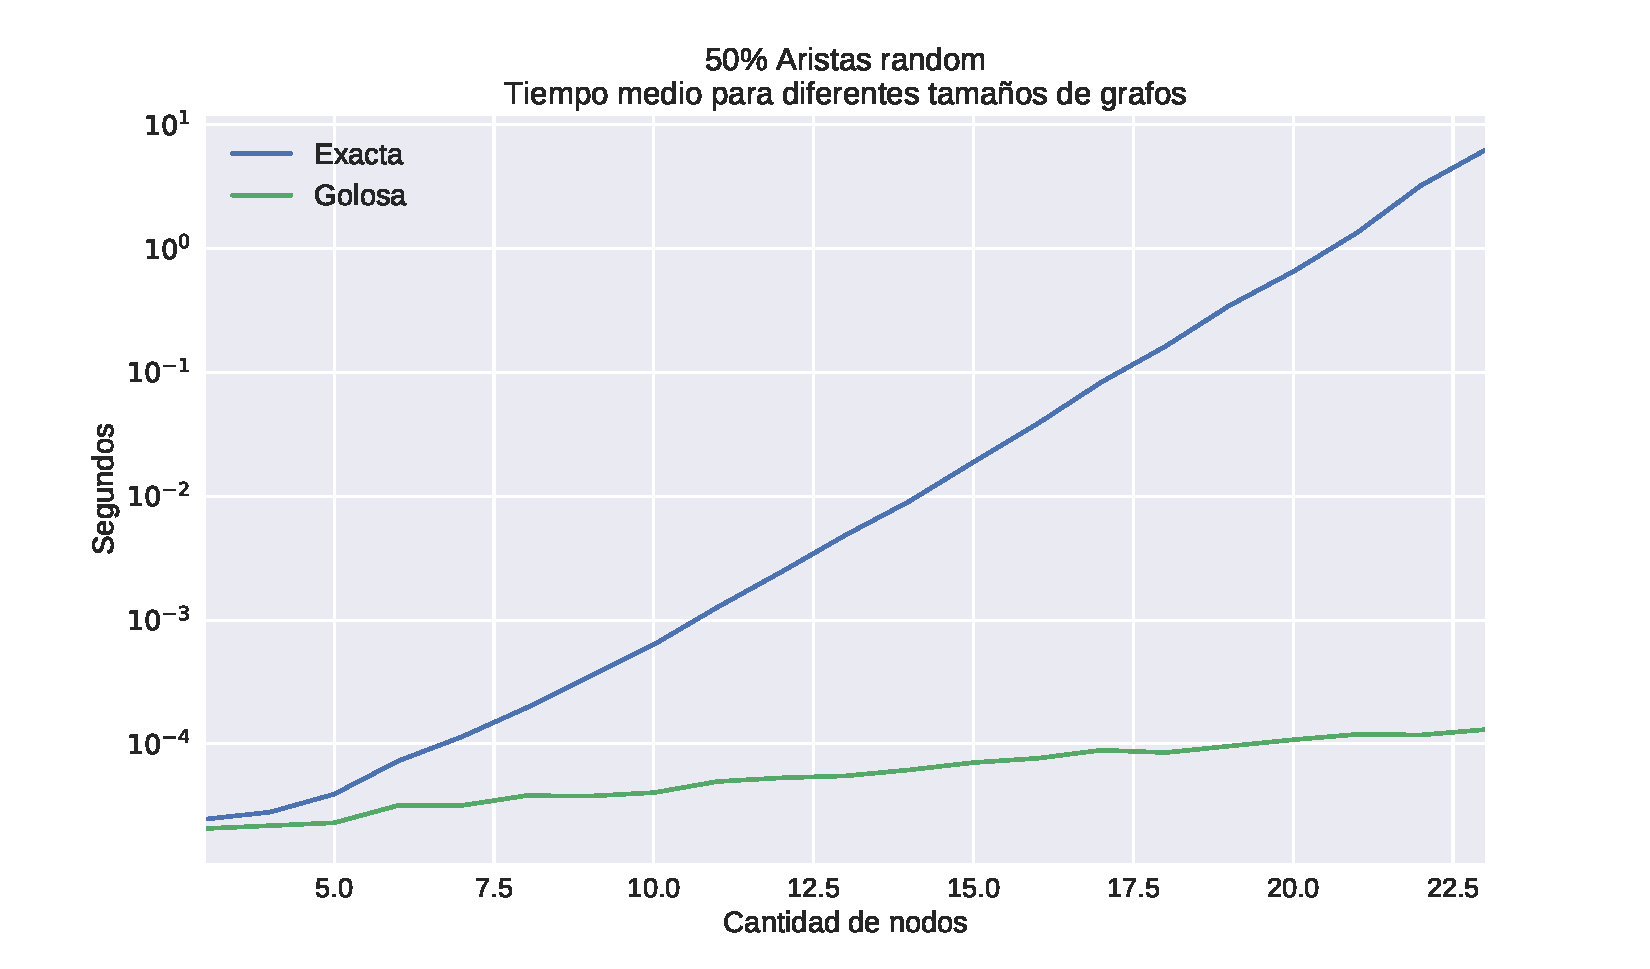
\includegraphics[width=1\textwidth]{informe/imgs/exp_random50_tiempo_greedy_exacta_logy.pdf} \\
%        \captionof{figure}{Escala logarítmica}
% }
% {\centering
%     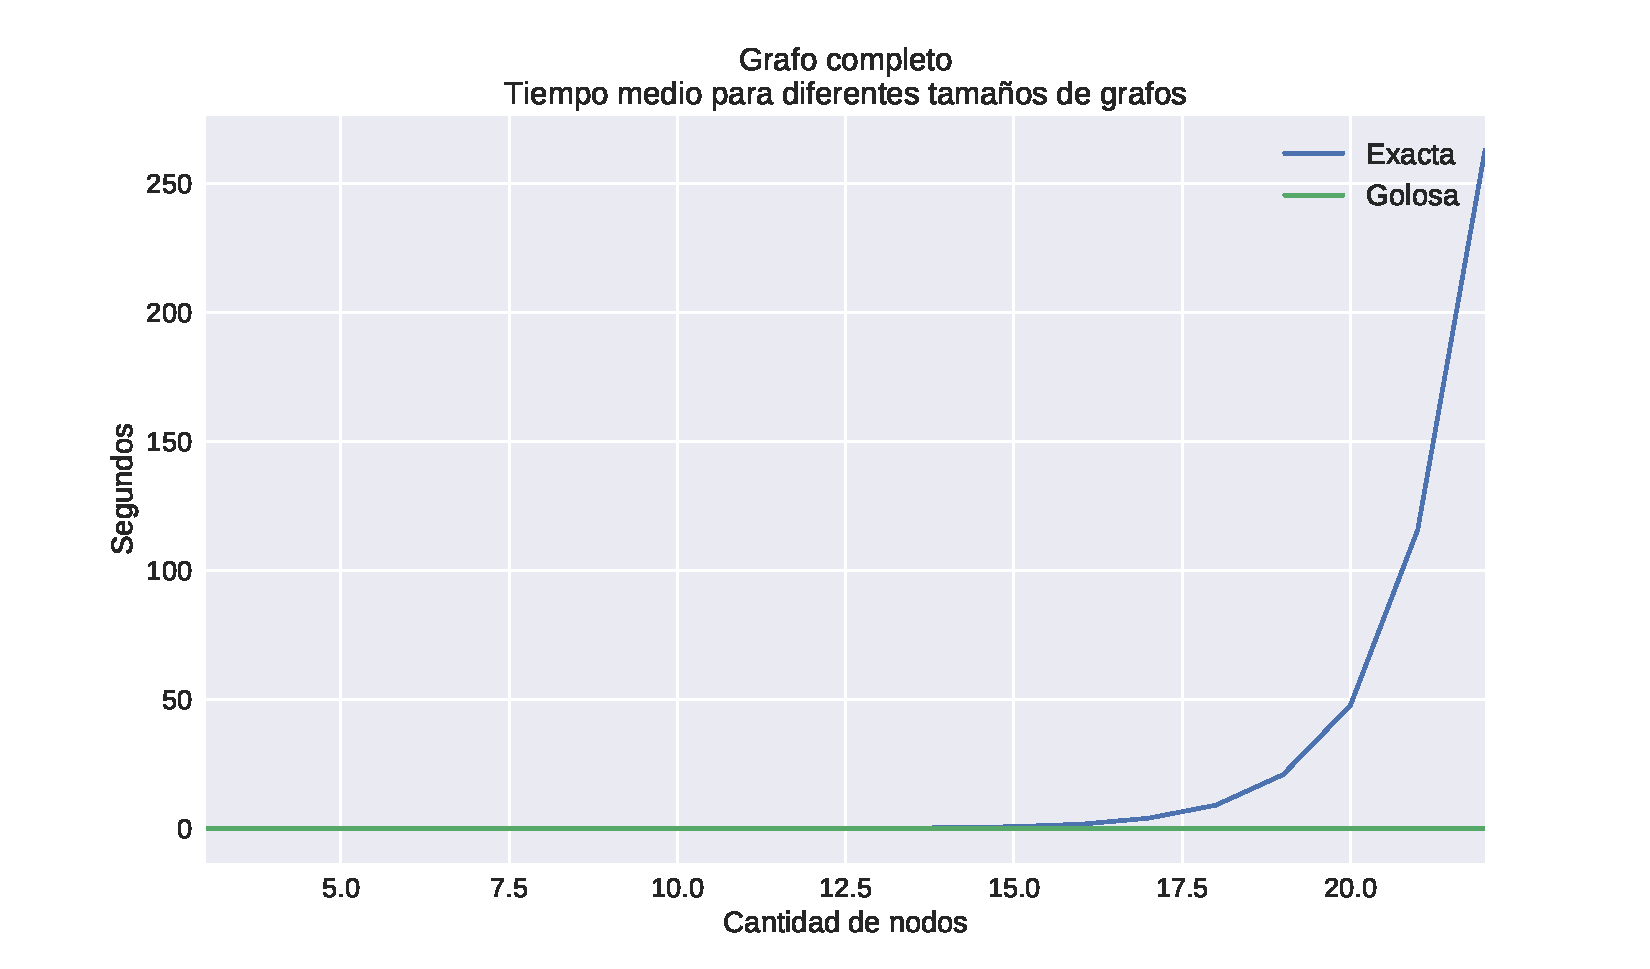
\includegraphics[width=1\textwidth]{informe/imgs/exp_completo_tiempo_greedy_exacta.pdf} \\
% }

La principal motivación de buscar heurísticas fue disminuir el tiempo de cómputo. Analizando la cota temporal teórica vimos que $O(n^5)$ es exponencialmente mejor que $O(2^{n} * n^{3})$. Veamos cómo son los tiempos en la práctica, considerando un grafo completo para el análisis de peor caso. \\

Dado que el algoritmo greedy es extremadamente rápido, decidimos mostrar un gráfico en \textbf{escala logarítmica} sobre los tiempos. Lo que puede verse es lo esperado.

{\centering
    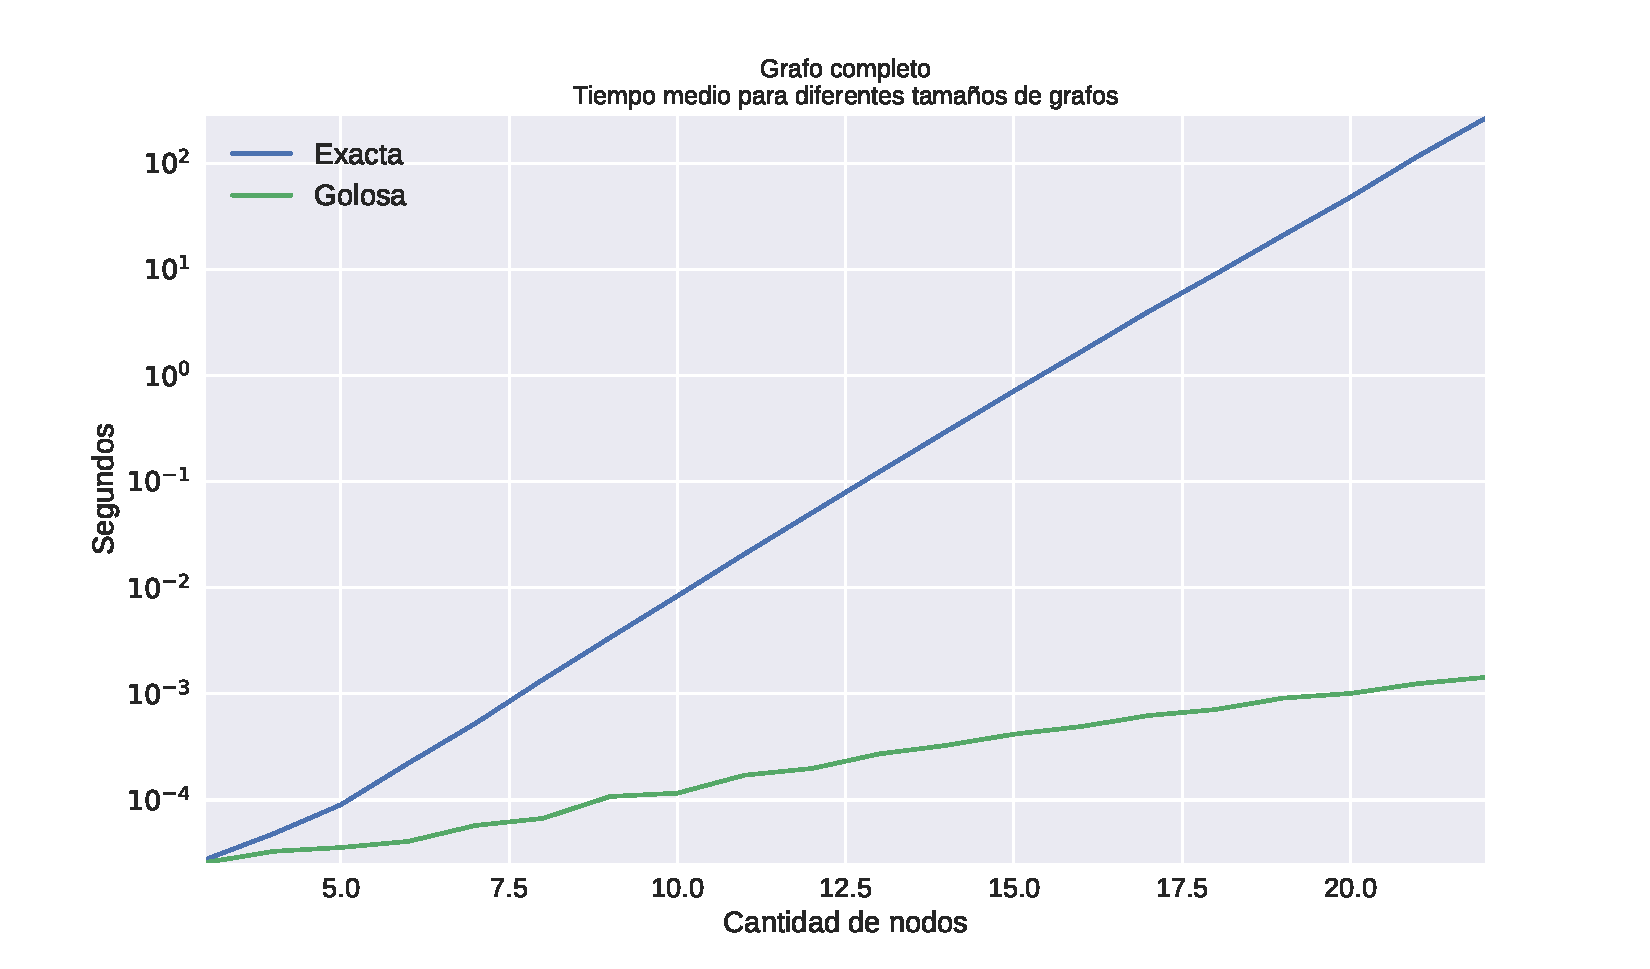
\includegraphics[width=1\textwidth]{informe/imgs/exp_completo_tiempo_greedy_exacta_logy.pdf} \\
    \captionof{figure}{$\uparrow$ Escala lagarítmica}
}

Si bien en el caso de los grafos completos, la frontera solución coincide con la óptima ($\#K_{n/2}$), el tamaño de la clique solución no es igual. Puede verse que el algoritmo greedy se queda con cliques más grandes que la estrictamente necesaria, y esto se debe a que la condición de selección incluye un $\geq$.

{\centering
    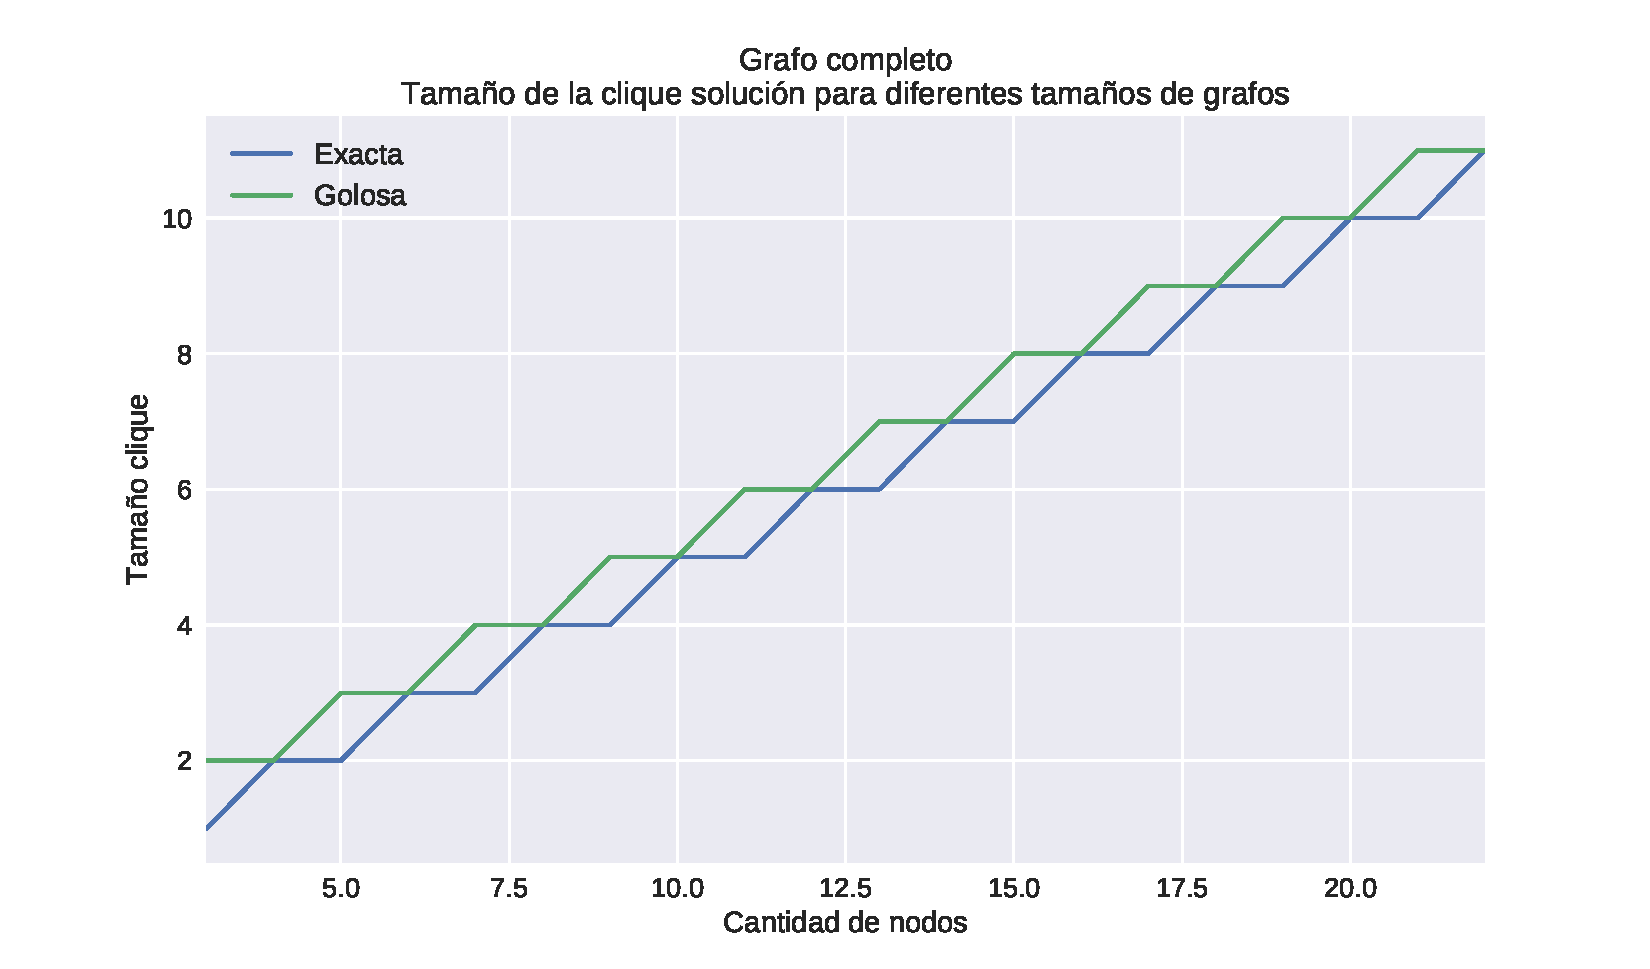
\includegraphics[width=1\textwidth]{informe/imgs/exp_completo_clique_greedy_exacta.pdf} \\
}

Retomando el análisis con los casos malos, habíamos mostrado que existen al menos un tipo de grafos (desde ahora simplemente \textbf{``grafos malos''}) donde la solución golosa podía estar tan lejos de la óptima como se quiera. Veamos gráficamente la diferencia en las soluciones. \\

{\centering
    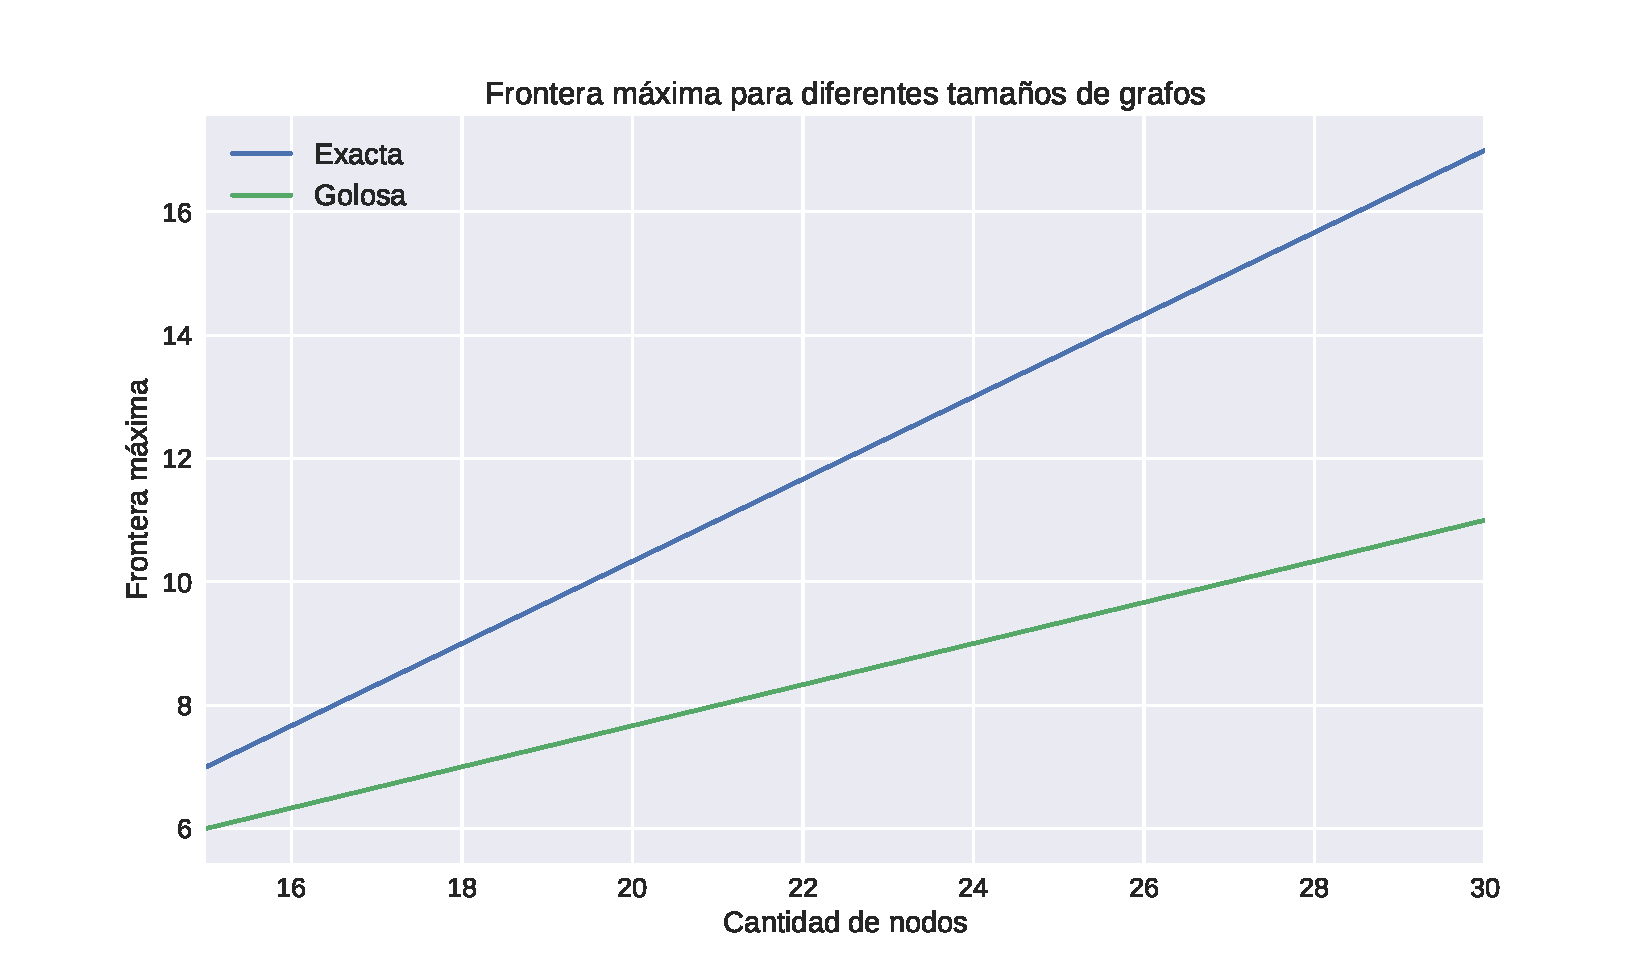
\includegraphics[width=1\textwidth]{informe/imgs/exp_malo_frontera_greedy_exacta.pdf} \\
    \captionof{figure}{$\uparrow$ Frontera para casos malos}
}
$ $\newline

Puede verse que a medida que $n$ crece, ambas soluciones se van alejando. No nos quedemos con la intuición, consideremos una demostración más formal: \\

Dado que estos ``grafos malos'' tienen su construcción bien definida, calculemos analíticamente cuál es el valor de la solución óptima para un tamaño de grafo $n$ dado. Esto nos será de utilidad para analizar optimalidad en secciones posteriores. \\

Como la solución óptima se encuentra en la clique formada por los nodos 2 y 3, consideremos el proceso de construcción. En cada paso se agregan 3 nodos, cada nuevo nodo como vecino de 1, 2 y 3 respectivamente. Podemos ver que 2 de cada 3 nodos contribuyen a aumentar nuestra solución inicial, por lo tanto, la solución óptima tiene que ser \textit{aproximadamente} $\frac{2}{3}n$, con alguna constante por los nodos iniciales. \\

Podemos comprobar empíricamente, observando los valores de frontera obtenidos por nuestro algoritmo exacto, que la solución óptima para ``grafos malos'' es exactamente $f(n) = \frac{2}{3}n - 3$. Este es un valor bien definido para $n$ divisibles por 3, dado que siempre los contruimos agregando 3 nodos por vez. \\

Con un razonamiento análogo, de cada 3 nodos que se agregan, un único nodo se agrega a lo que será la solución golosa. De hecho, puede verse que la solución golosa para un grafo malo es exactamente $g(n) = \frac{1}{3}n + 1$, también bien definido para $n$ divisibles por 3. \\

Veamos finalmente qué sucede con la diferencia entre ambas soluciones a medida que crece $n$:

$$g(n) - f(n)$$
$$(\frac{2}{3}n - 3) - (\frac{1}{3}n + 1)$$
$$\frac{2}{3}n - 3 - \frac{1}{3}n - 1$$
$$\frac{1}{3}n - 4$$
\[ \lim_{x \to \infty} (\frac{1}{3}n - 4) = \infty \] \qed \\

Demostramos entonces que la diferencia entre la solución óptima y la solución greedy para un mismo grafo puede ser arbitrariamente grande. Es decir, dado un $n$ lo suficientemente grande las soluciones pueden ser tan diferentes como uno quiera. La motivación de las siguientes heurísticas será intentar de mejorar las soluciones en los grafos malos, para intentar acercarnos lo más posible al óptimo. \\

Para finalizar este apartado, es importante notar que en promedio el algoritmo greedy da resultados razonablemente buenos, sobre todo teniendo en cuenta el mínimo costo computacional que tiene asociado. Veremos más sobre casos promedios al final del informe, donde realizaremos una comparación entre las diferentes heurísticas. \\
